% Simple poster (portrait)
% Author: Sofia Jijon (https://sjijon.github.io)
% Last Update: Sept 9, 2021
% Latest Version: https://github.com/sjijon/TeX-templates/tree/main/Tikzposter%20posters/Simple%20poster

\documentclass[a0paper,portrait,margin=0pt, colspace=24pt,subcolspace=0pt,blockverticalspace=36pt,innermargin=50pt]{tikzposter}

\usepackage[latin9]{inputenc}
\usepackage[square,numbers]{natbib} 	% Bibliography manager
\usepackage{amsmath,amssymb}
\usepackage{lipsum}  				    % Random Text
\usepackage[colalign]{aligncolsatbottom}  %To align columns at bottom (!! please run 2 times)

%..............................................................................................................................................................................................
% Display
\tikzposterlatexaffectionproofoff 			
\usetikzlibrary{shapes.geometric,arrows.meta,positioning}  %Tikz Libraries

% Fonts
\usepackage{helvet}					% Sans-Serif
\renewcommand{\familydefault}{\sfdefault}	%

% Colors
	\definecolor{MyOrange}{rgb}{0.8, 0.33, 0}
	\definecolor{MyBrown}{rgb}{0.28, 0.20, 0.20}
        %r: 167; g: 197; blue: 232
        %r: .65; g: 0.77; blue: 0.90
        \definecolor{MyBlueLight}{rgb}{0.65, 0.77, 0.90}
        %r: 22; g: 31; blue: 129
        %r: .08; g: 0.12; blue: 0.50
        \definecolor{MyBlueDark}{rgb}{0.08, 0.12, 0.5}
	\definecolor{MyGreen}{rgb}{0.33, 0.42, 0.18}

% Theme
\usetheme{Default}
\definecolorstyle{MyStyle2016}{
	\definecolor{ColorOne}{named}{MyBlueLight} 
	\definecolor{ColorTwo}{named}{MyBlueDark}
	\definecolor{ColorThree}{named}{MyGreen}
}{
    % Title Colors
    \colorlet{titlebgcolor}{ColorOne}
    \colorlet{titlefgcolor}{white}
    % Background Colors
    \colorlet{backgroundcolor}{ColorOne!15}
    \colorlet{framecolor}{ColorOne}
    % Block Colors
    \colorlet{blocktitlebgcolor}{white}
    \colorlet{blocktitlefgcolor}{ColorTwo}
    \colorlet{blockbodybgcolor}{white}
    \colorlet{blockbodyfgcolor}{black}
    % Innerblock Colors
    \colorlet{innerblocktitlebgcolor}{ColorOne!15}
    \colorlet{innerblocktitlefgcolor}{black}
    \colorlet{innerblockbodybgcolor}{ColorOne!15}
    \colorlet{innerblockbodyfgcolor}{black}
    % Note colors
    \colorlet{notebgcolor}{ColorTwo!20}
    \colorlet{notefgcolor}{ColorTwo}
    \colorlet{notefrcolor}{ColorTwo}
 }

% Color style
\usecolorstyle{MyStyle2016}
%..............................................................................................................................................................................................
%\title{Modelling A Limb Congruency Learning Task}
\title{How does false visual input affect learning in sensorimotor adaption?}

\author{Antonio Amaddio}

\institute{FU-Berlin, Department of Psychology}

%..............................................................................................................................................................................................
\begin{document}
%
%
%	HEAD
%
%....................................................................................
%
%	Title
%
\maketitle[width=0.96\linewidth,titletoblockverticalspace=36pt,linewidth=0,roundedcorners=10]
%..............................................................................................................................................................................................
%
%	LEFT COLUMN
%
\begin{columns}
\column{0.33}
%....................................................................................
%
%	Block
%
\block [titleleft,roundedcorners=16]{1. Research Question}{
        \raggedright
        \textbf{Sensorimotor Adaptation}: Humans can learn/update a movement to adjust to changes from sensory input. \\
        \mbox{} \\
        Learning of \textbf{motor actions} is driven by \textbf{error processing}. Feedback of information from proprioception and vision is integrated \textbf{when the two are congruent}. \\
        \mbox{} \\ \textbf{Vision outweighs proprioception} due to its higher spatial accuracy. But how does this mechanism affect the learning rate? \\

        RQ: How well do humans learn a new movement when the visual feedback is wrong?
}
%....................................................................................
%
%	Block
%
\block[titleleft,roundedcorners=16]{2. Experimental Set-Up}{
    %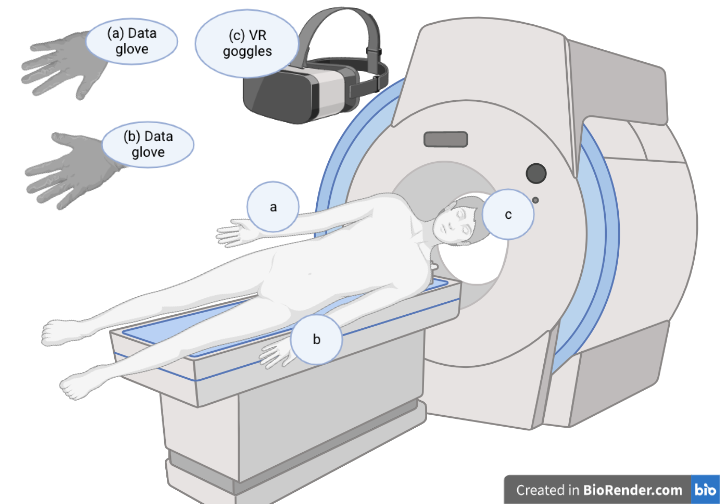
\includegraphics[width=\linewidth]{Seminar Poster/Figures/experiment-set-up.png}
    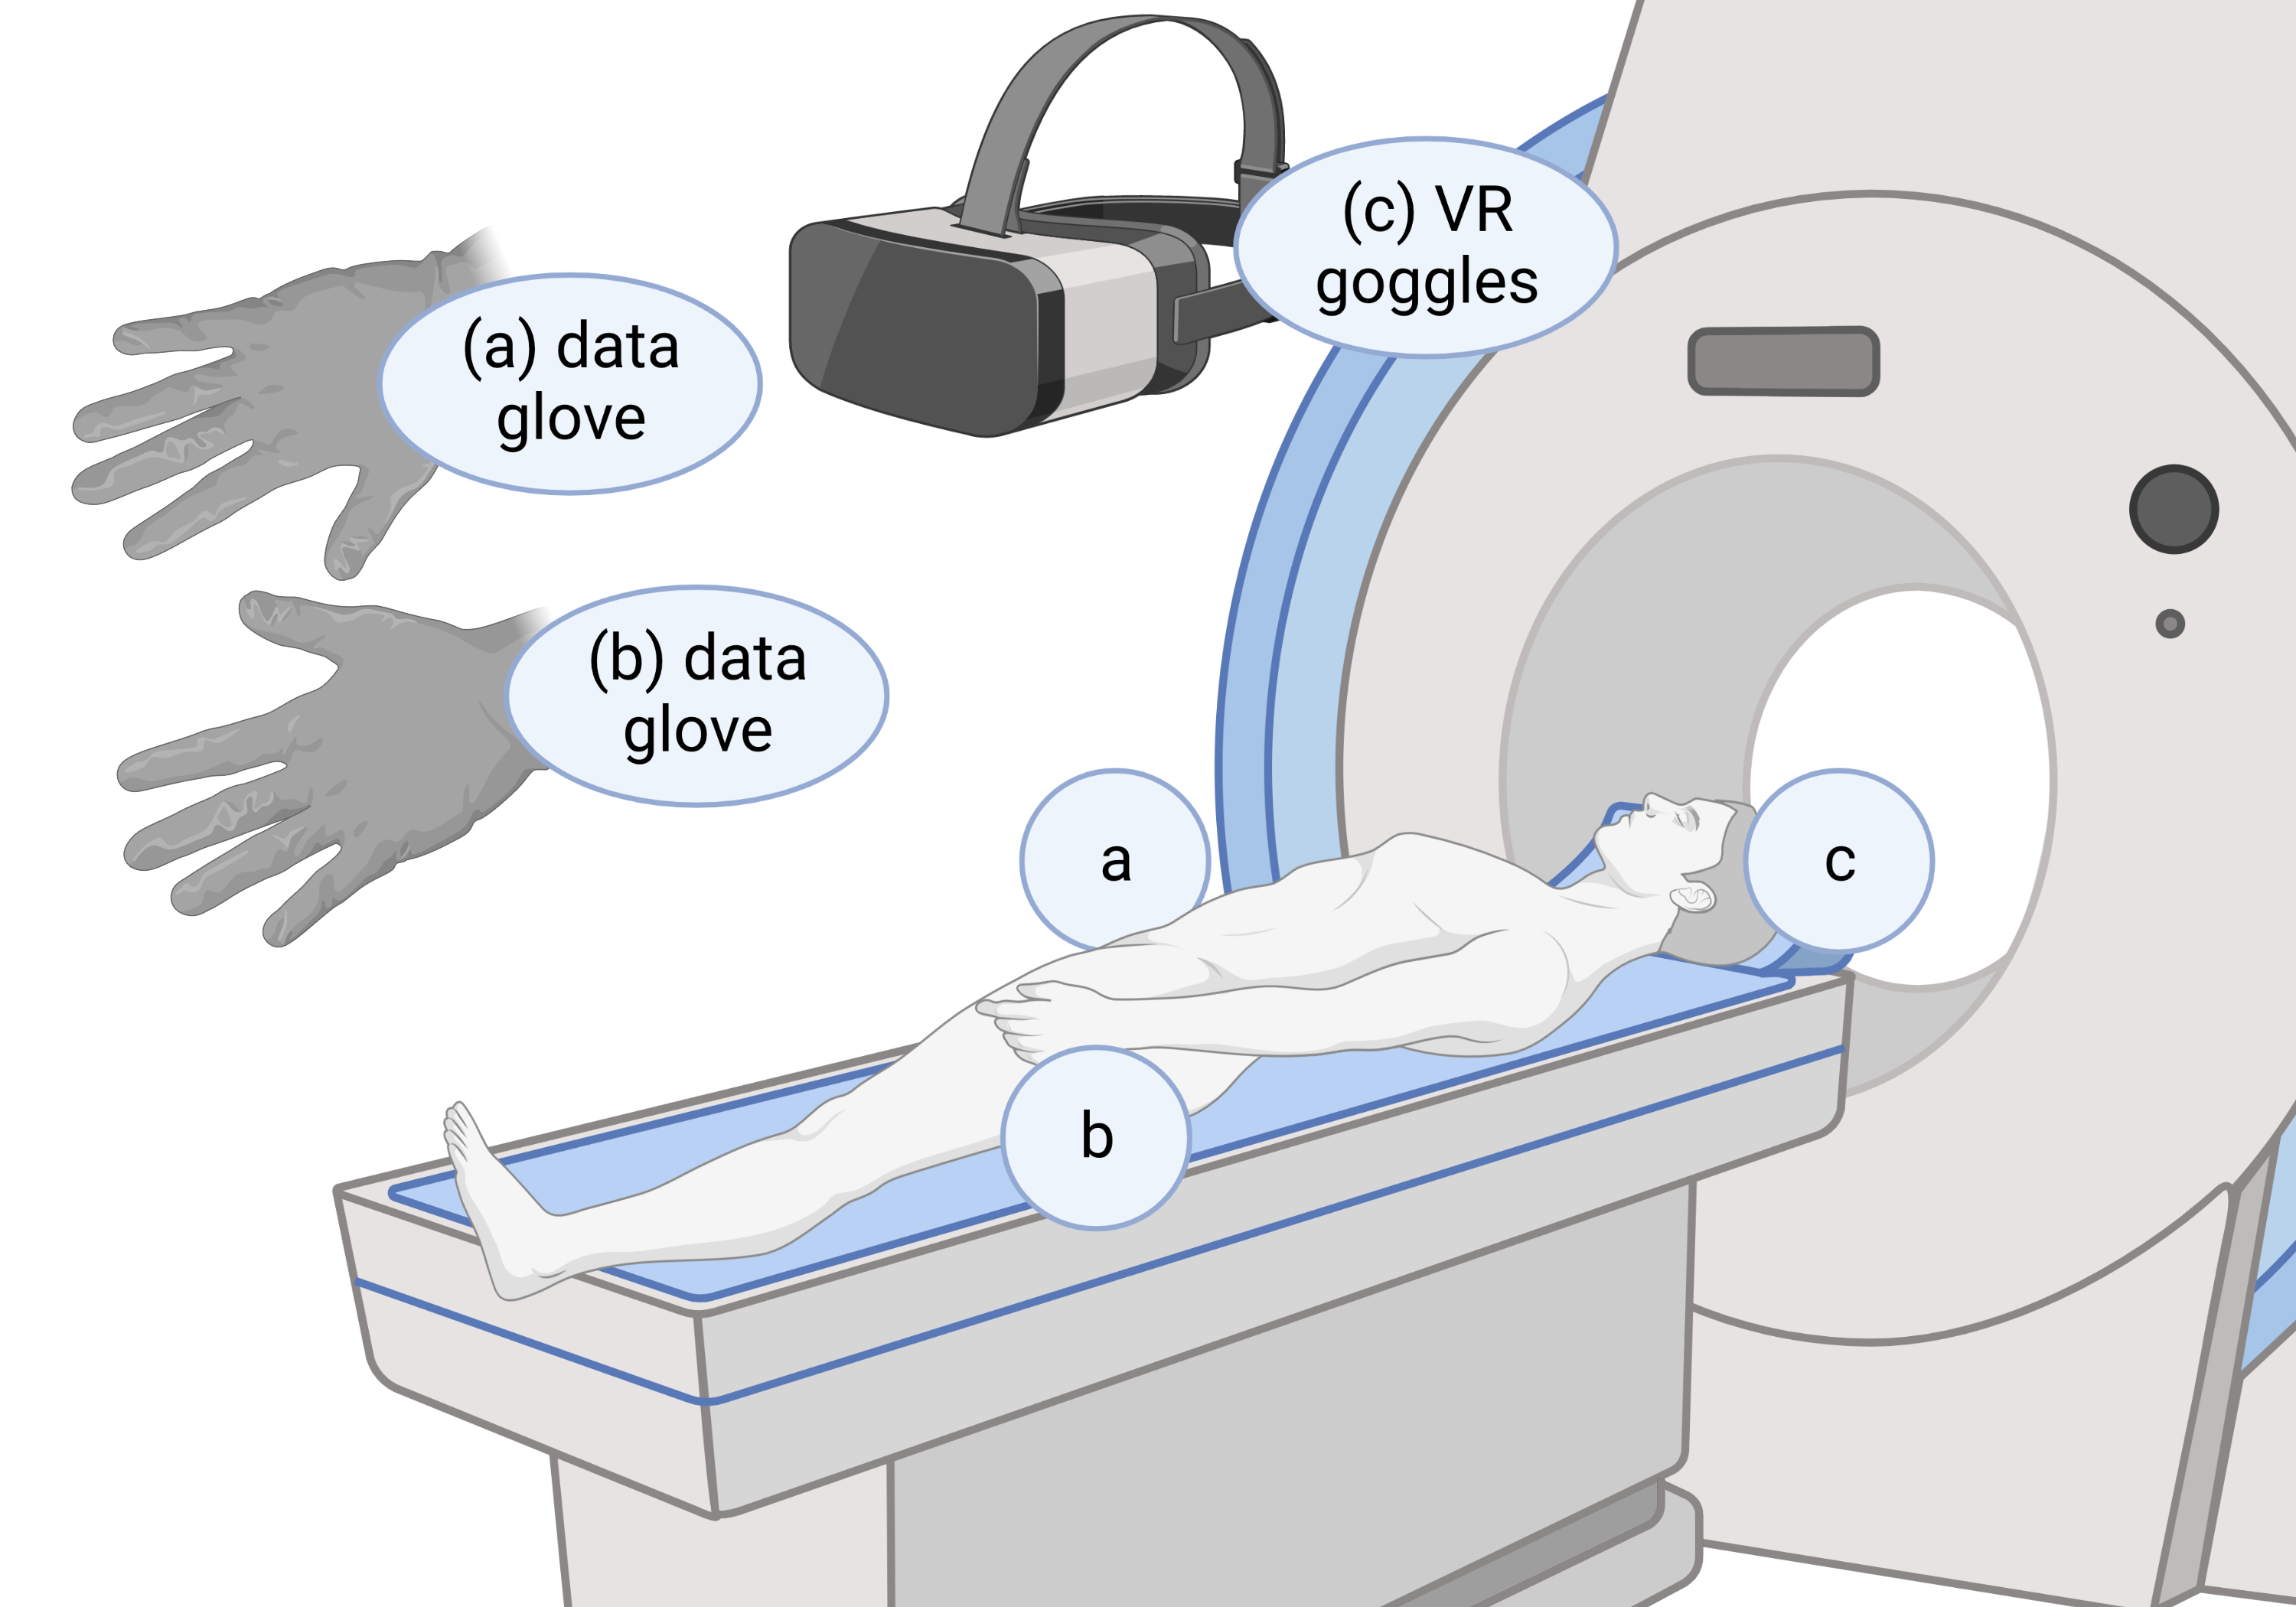
\includegraphics[width=\linewidth]{Seminar Poster/Figures/experiment-set-up-zoomed-side.png}
}
%....................................................................................
%
%	Block
%
\block[titleleft,roundedcorners=16]{3. Experimental Task}{
	\raggedright
	A finger movement task where (healthy) subjects \textbf{perform better over time}, naturally. \\
        \mbox{} \\ \textbf{Preparation}: (1) Cross hands, (2) grasp each other, (3) twist wrists vertically. \\
        \mbox{} \\ \textbf{Instruction}: Move finger arrow is pointing to (VR googles; see c above). \textbf{No correction} allowed.\\ 
	%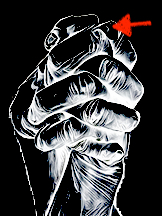
\includegraphics{Seminar Poster/Figures/crossed-hands-sketch-whitespace-removed-small-w-arrow.jpeg}
	%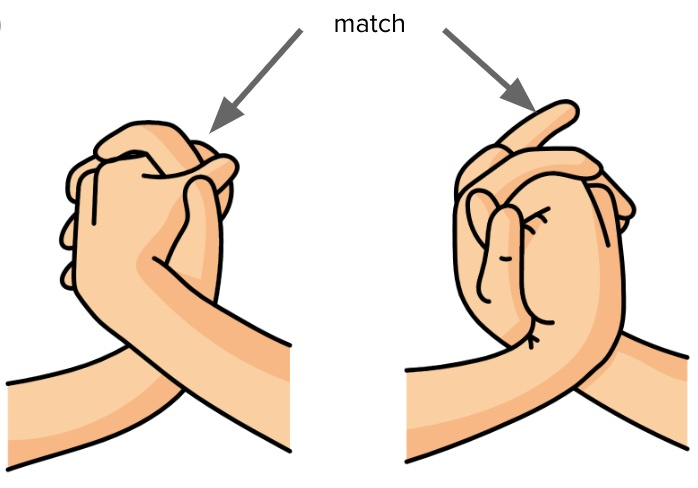
\includegraphics{Seminar Poster/Figures/task-meme.jpg}
	\begin{minipage}{0.1\textwidth}
	    \raggedright
	    Any finger can be randomly chosen ($p=.1$). Virtual observed 3D hands/fingers (Goggles; see c above) are synched with subject's limbs (Data glove; see a, b above).
	\end{minipage}
        \begin{minipage}{0.15\textwidth}
	    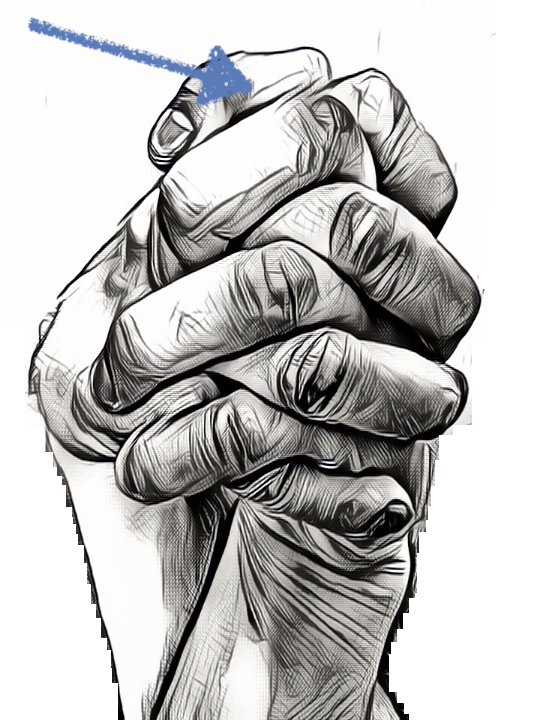
\includegraphics[width=\textwidth]{Seminar Poster/Figures/crossed-hands-sketch-b-on-w-with-arrow.jpeg}
	\end{minipage}
	\noindent
}
%..............................................................................................................................................................................................
%
%	CENTER COLUMN
%
%\column{0.34}
\column{0.67}
%....................................................................................
%
%	Block
%
\block[titleleft,roundedcorners=16]{4. Experimental Design}{
 \raggedright
 \textbf{Learning} will be \textbf{manipulated} experimentally by visual correct/incorrect feedback.
 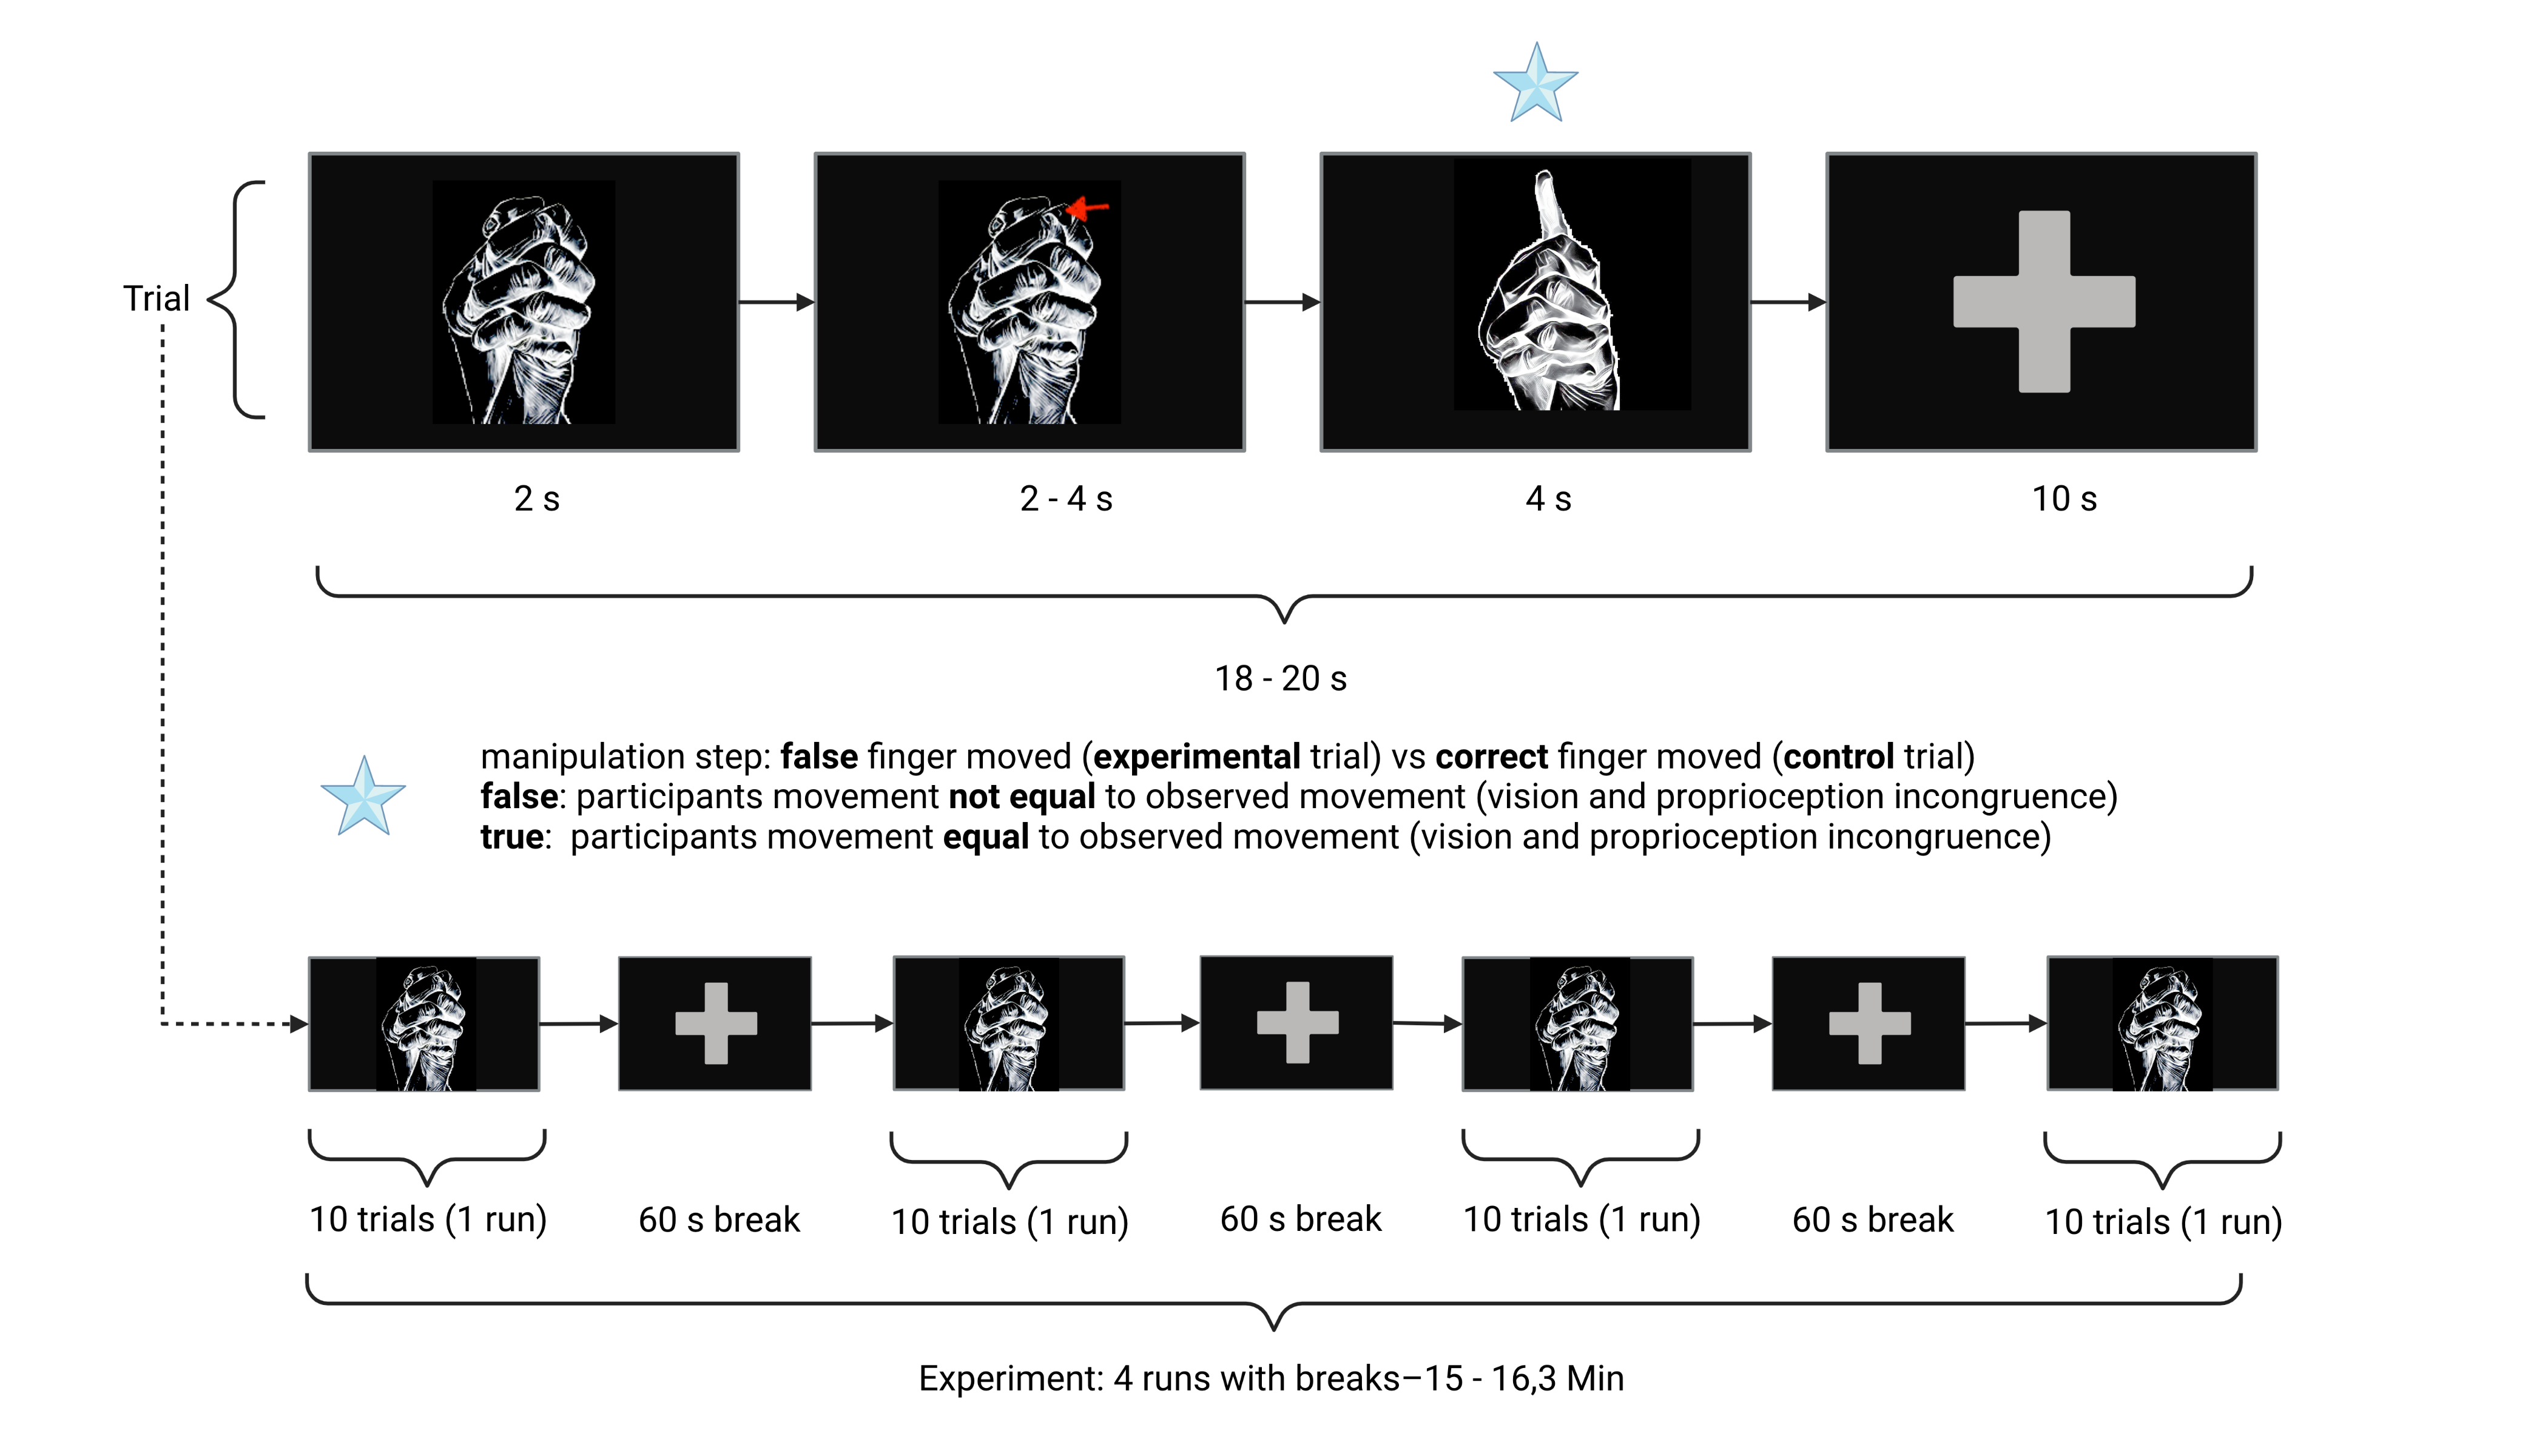
\includegraphics[width=\linewidth]{Seminar Poster/Figures/experiment-runs.png}
}
%....................................................................................
%
% 	Block
%
\block[titleleft,roundedcorners=16]{7. Region of Interests}{    
	\begin{minipage}{0.5\linewidth}
	    \textbf{EBA}: Congruent versus incongruent visual and proprioceptive information. \\
            \mbox{} \\
            \textbf{DLPFC}: Activated in early learning processes. Shift from automatic to cognitive control. State: Consciously (implicitly) learning. \\
            \mbox{} \\
            \textbf{Cerebellum}: Activated in late learning processes. Shift from cognitive controlled to automatically retrieved motor action. State: Motor action has been learned.
	\end{minipage}
	\begin{minipage}{0.5\linewidth}
	    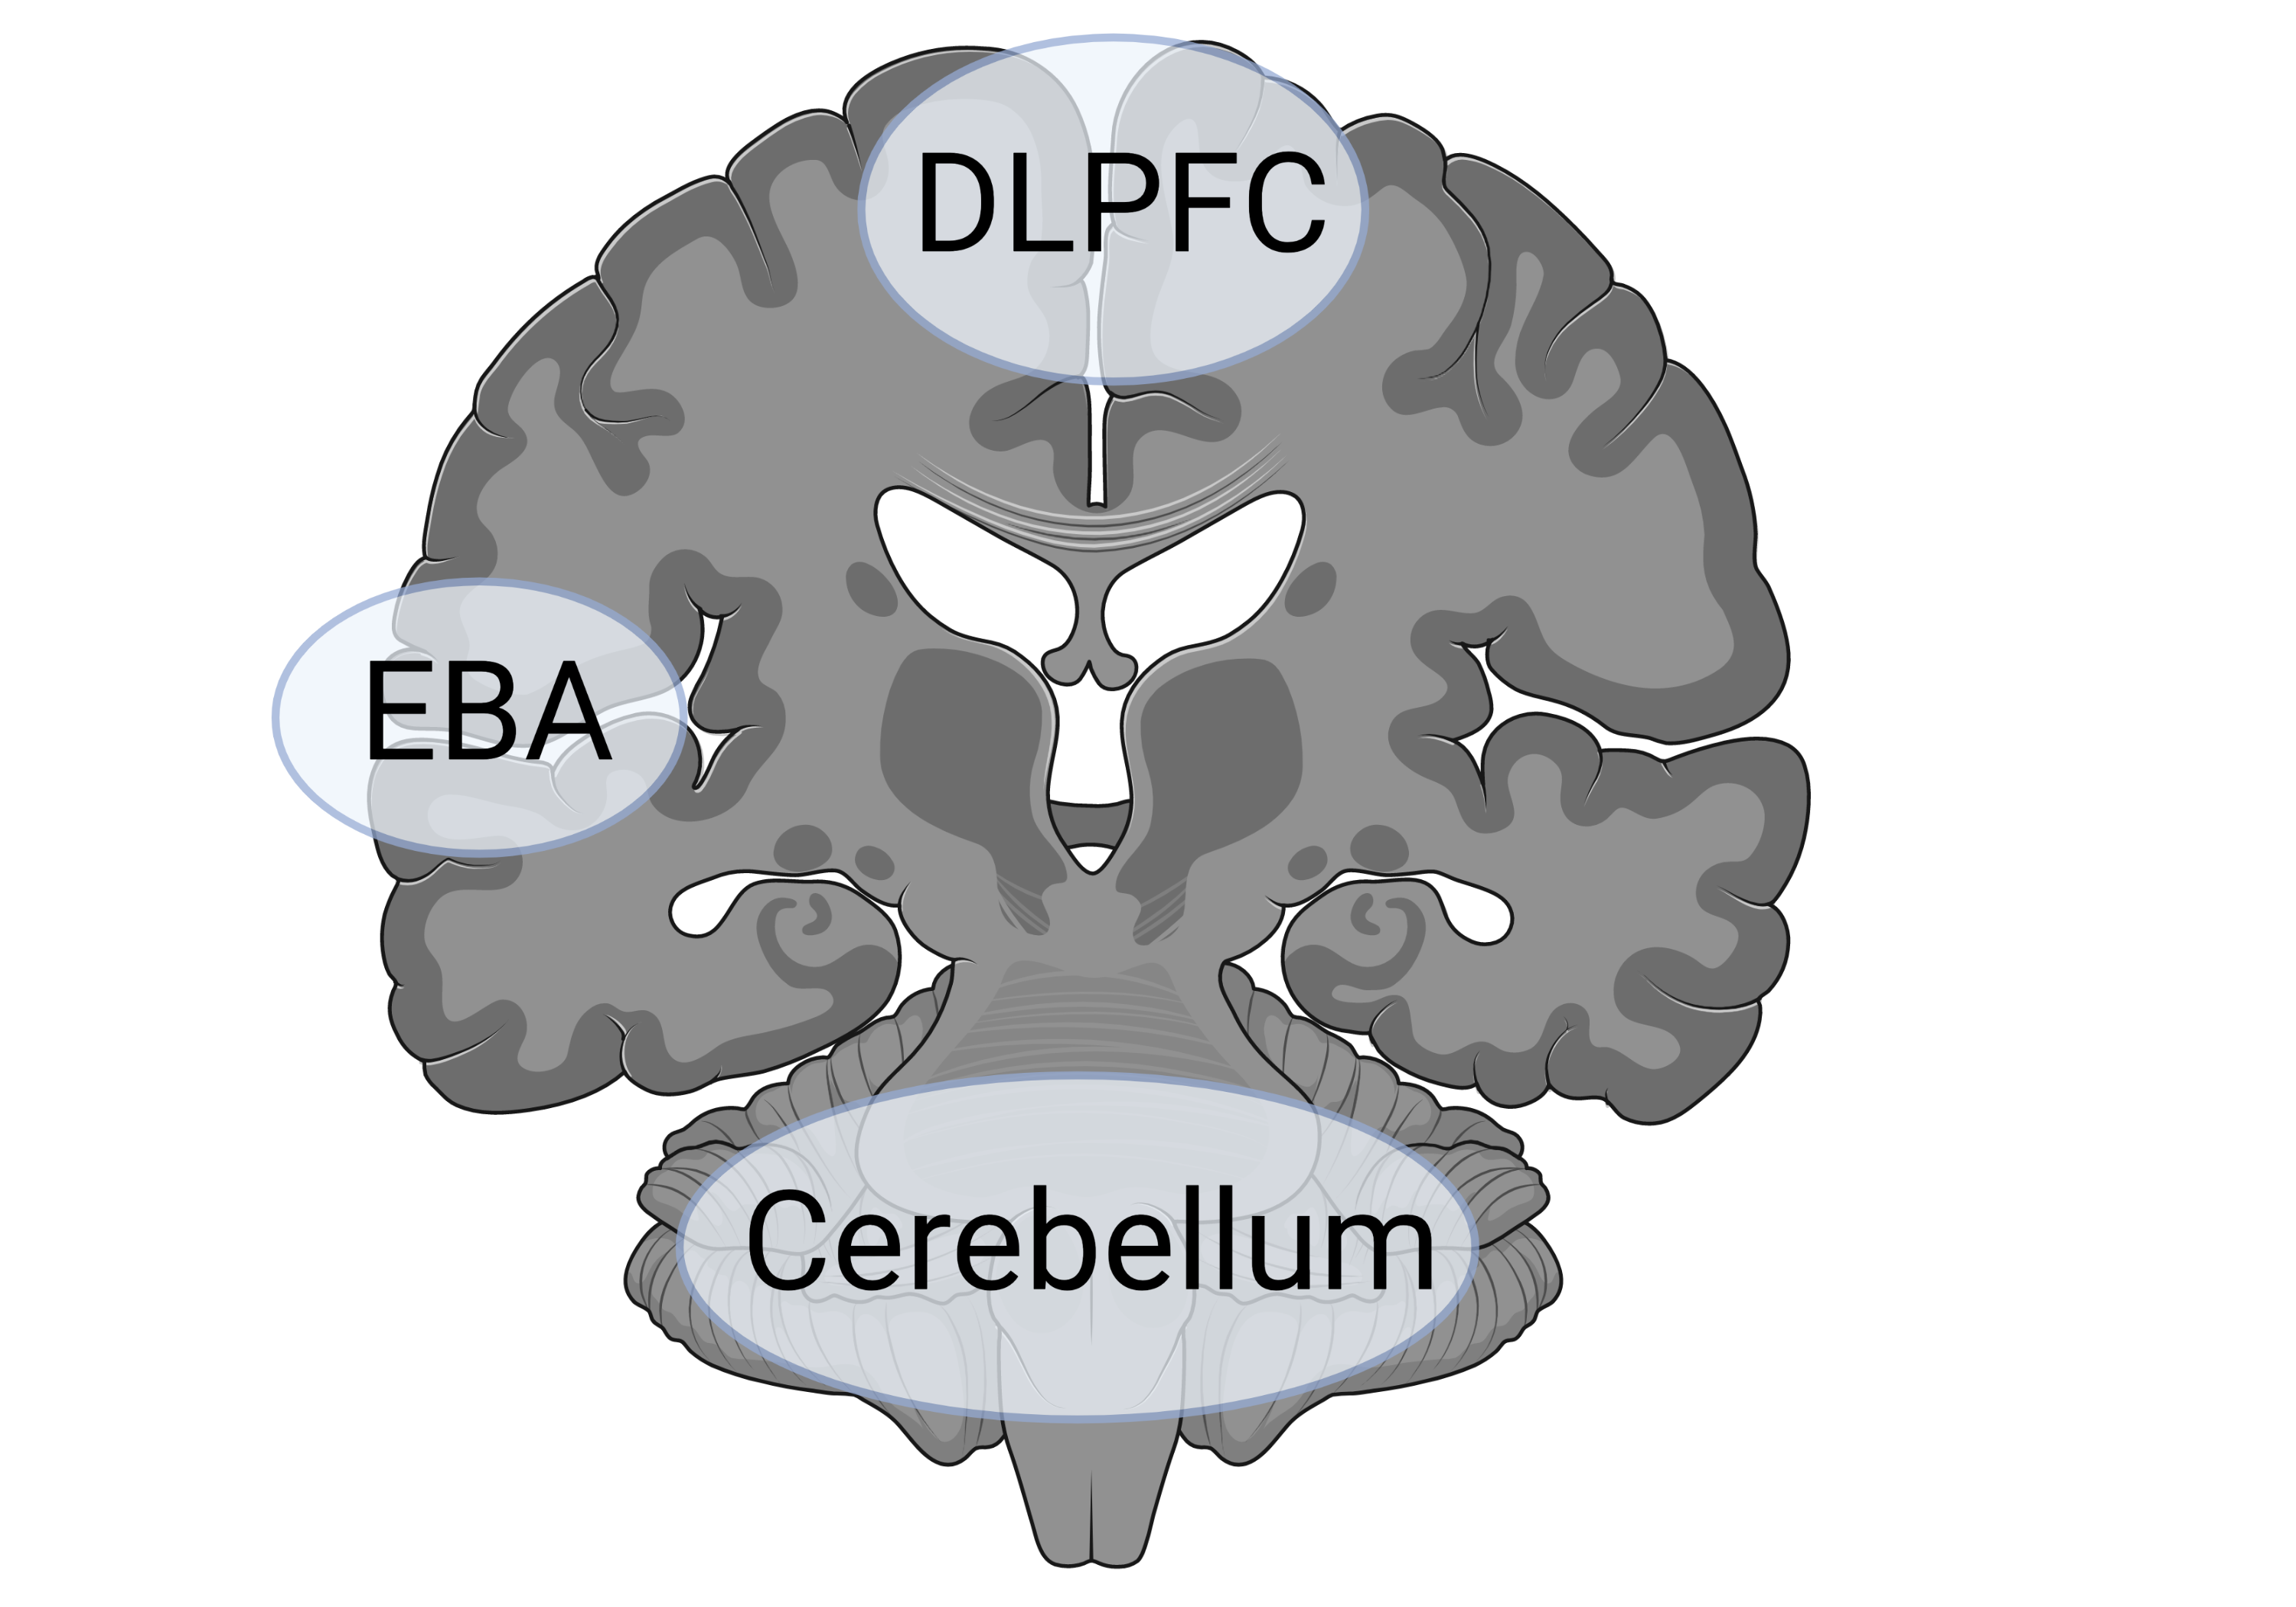
\includegraphics[width=0.49\linewidth]{Seminar Poster/Figures/coronar-brain-slice.png}
            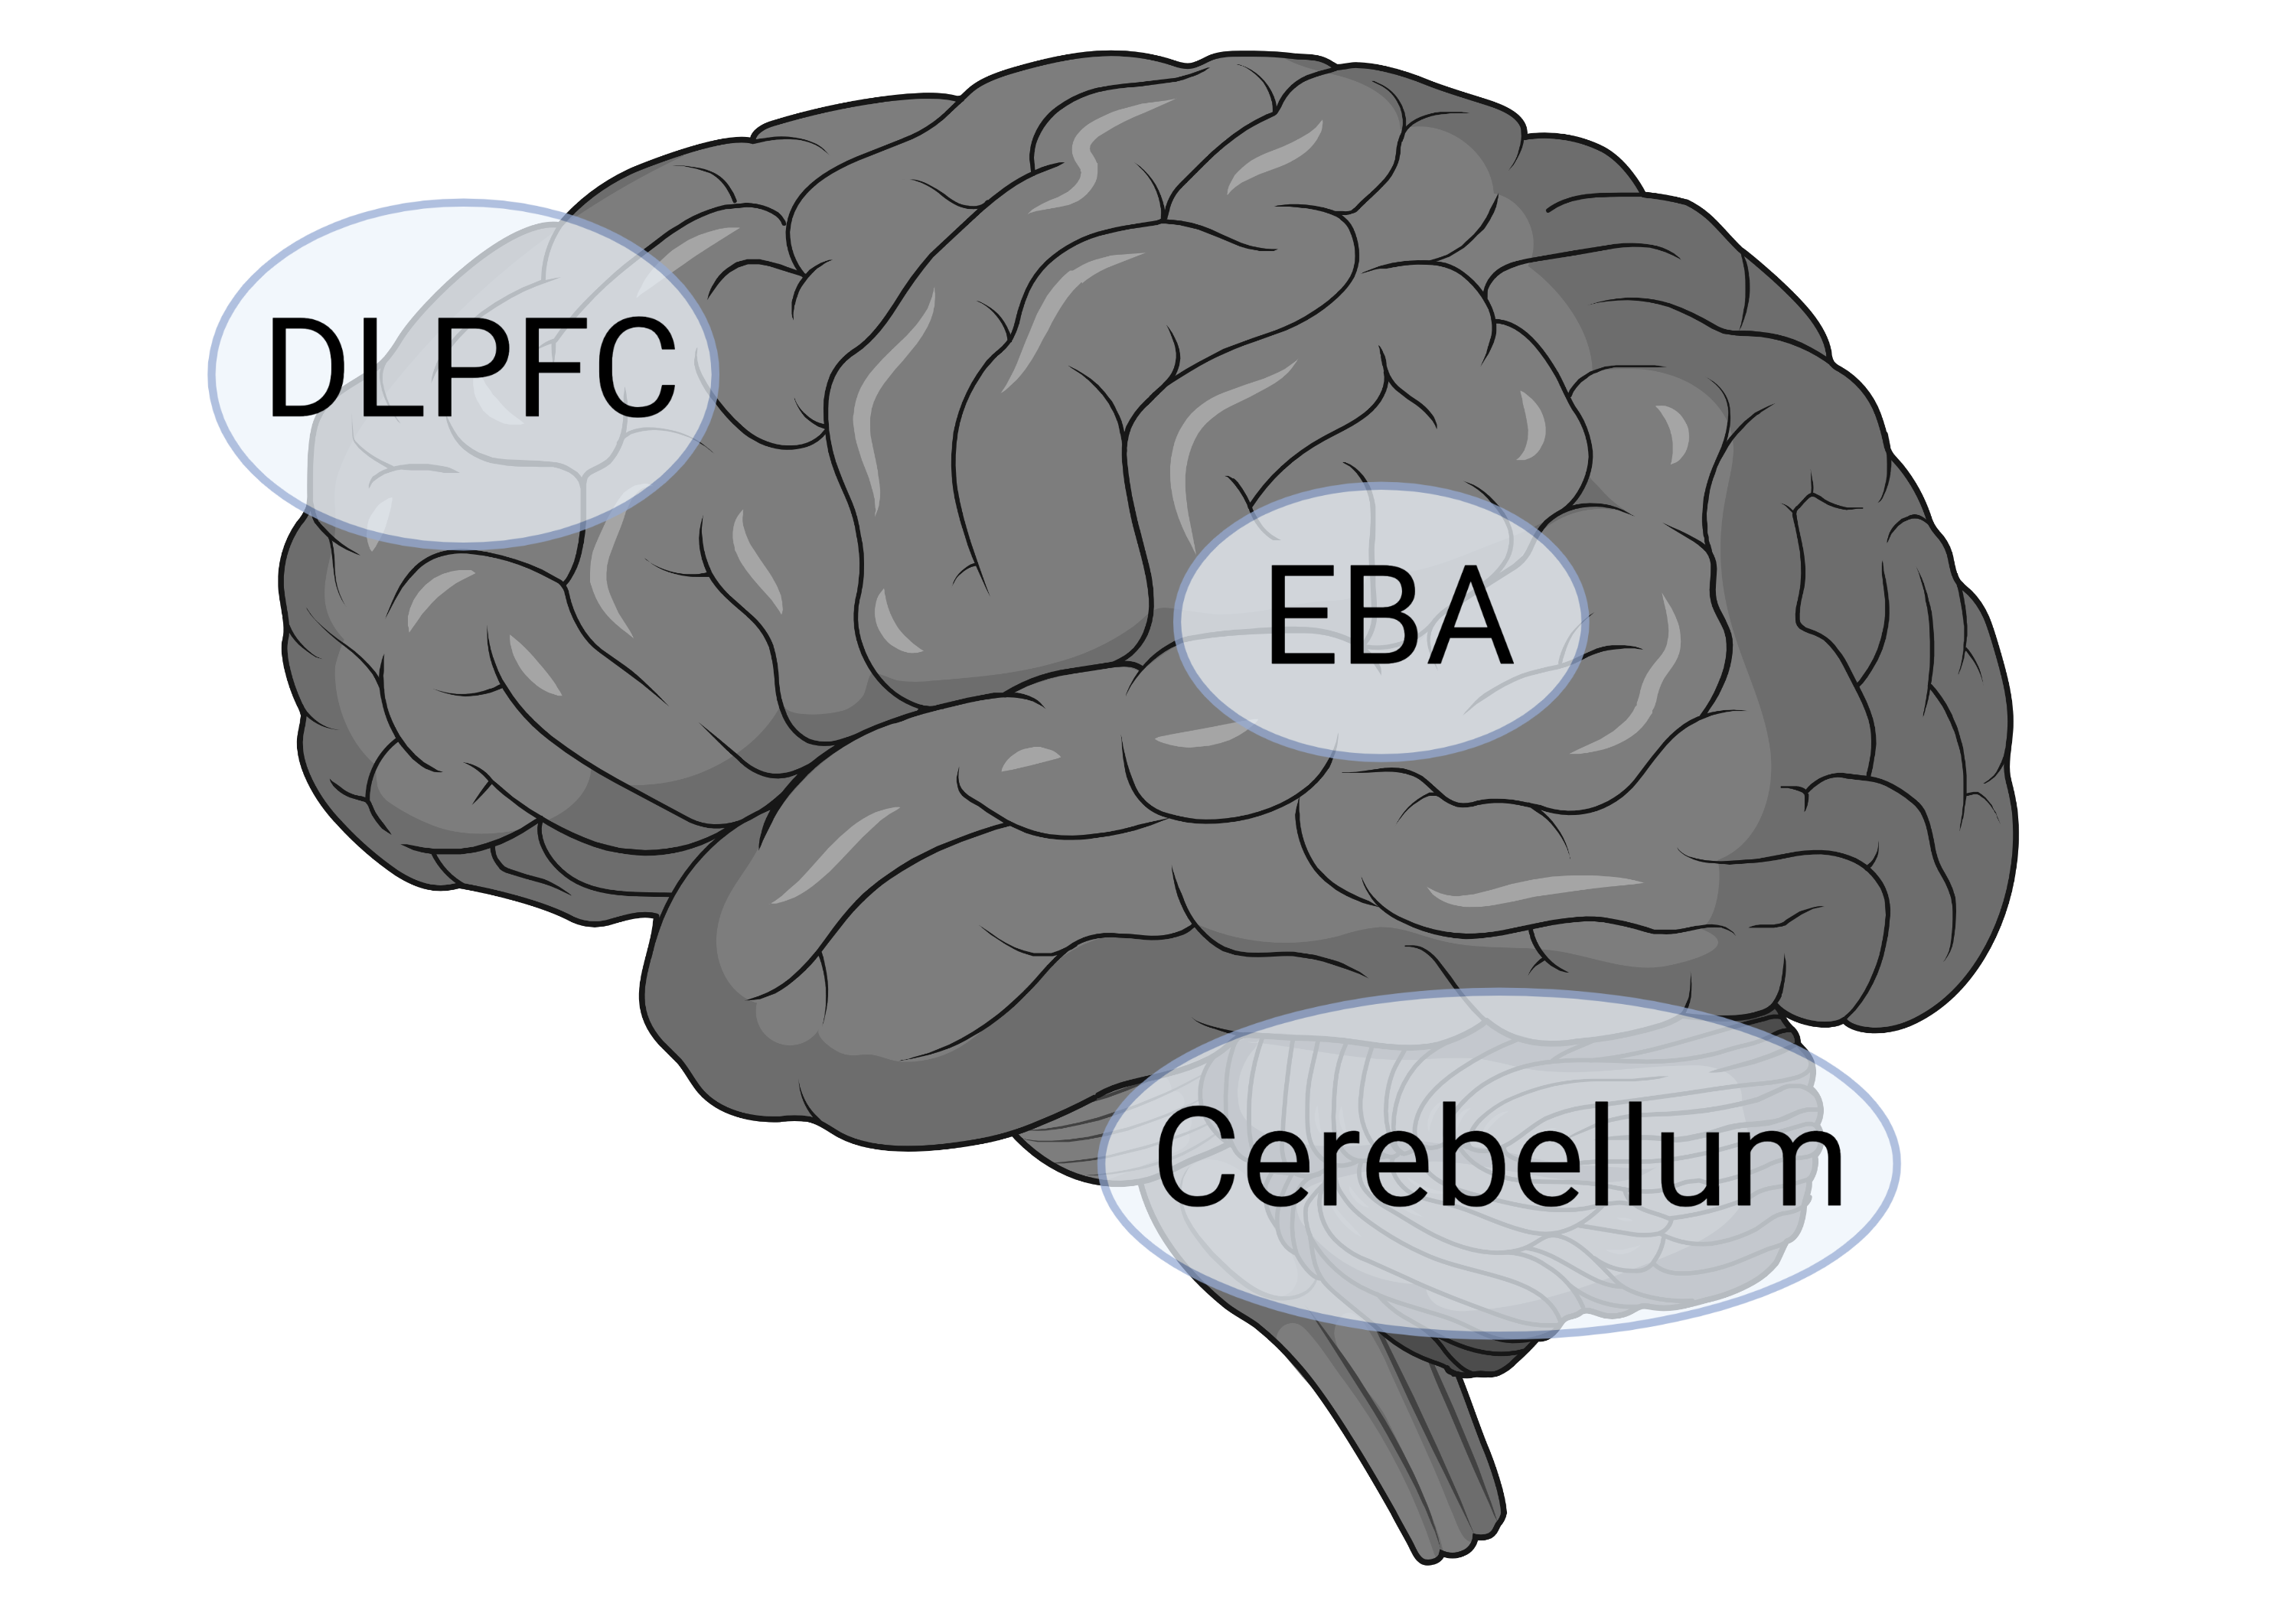
\includegraphics[width=0.49\linewidth]{Seminar Poster/Figures/lateral-brain.png}
	\end{minipage}
	
}
%....................................................................................
%
%	Block
%
\block[titleleft,roundedcorners=16]{5. Expected Learning Models}{
 Expected learning models when the visual feedback \textbf{is false}. Learning = move correct finger.
    \mbox{}\\
    \begin{itemize}
        \item \textbf{Hinderance}: slower learning.
        \item \textbf{Overwrite}: no learning.        
        \item \textbf{Resilience}: (uninhibited) learning. Humans learn irrelevant the correctness of the visual feedback.
    \end{itemize}
}
%....................................................................................
%
%	Block
%
%\block[titleleft,roundedcorners=16]{6. Unexpected Learning Models}{
% Potential learning models when the visual feedback \textbf{is false}.
%    \mbox{}\\
%    \begin{itemize}
%        \item \textbf{Confidence}: Active early learning, then no learning and relying on old learned model. Humans integrate external sensory information for as long as they trust it.
%        \item \textbf{Random}: Active early learning, then no learning and guessing. Humans move a random finger, when they can not trust either inner nor external sensory input.
%    \end{itemize}
%}
%..............................................................................................................................................................................................
%
% 	RIGHT COLUMN
%
%\column{0.33}
%....................................................................................
%
%	Block
%
\block[titleleft,roundedcorners=16]{8. Neurocognitive Learning Models }{
    \textbf{Hinderance} \\
    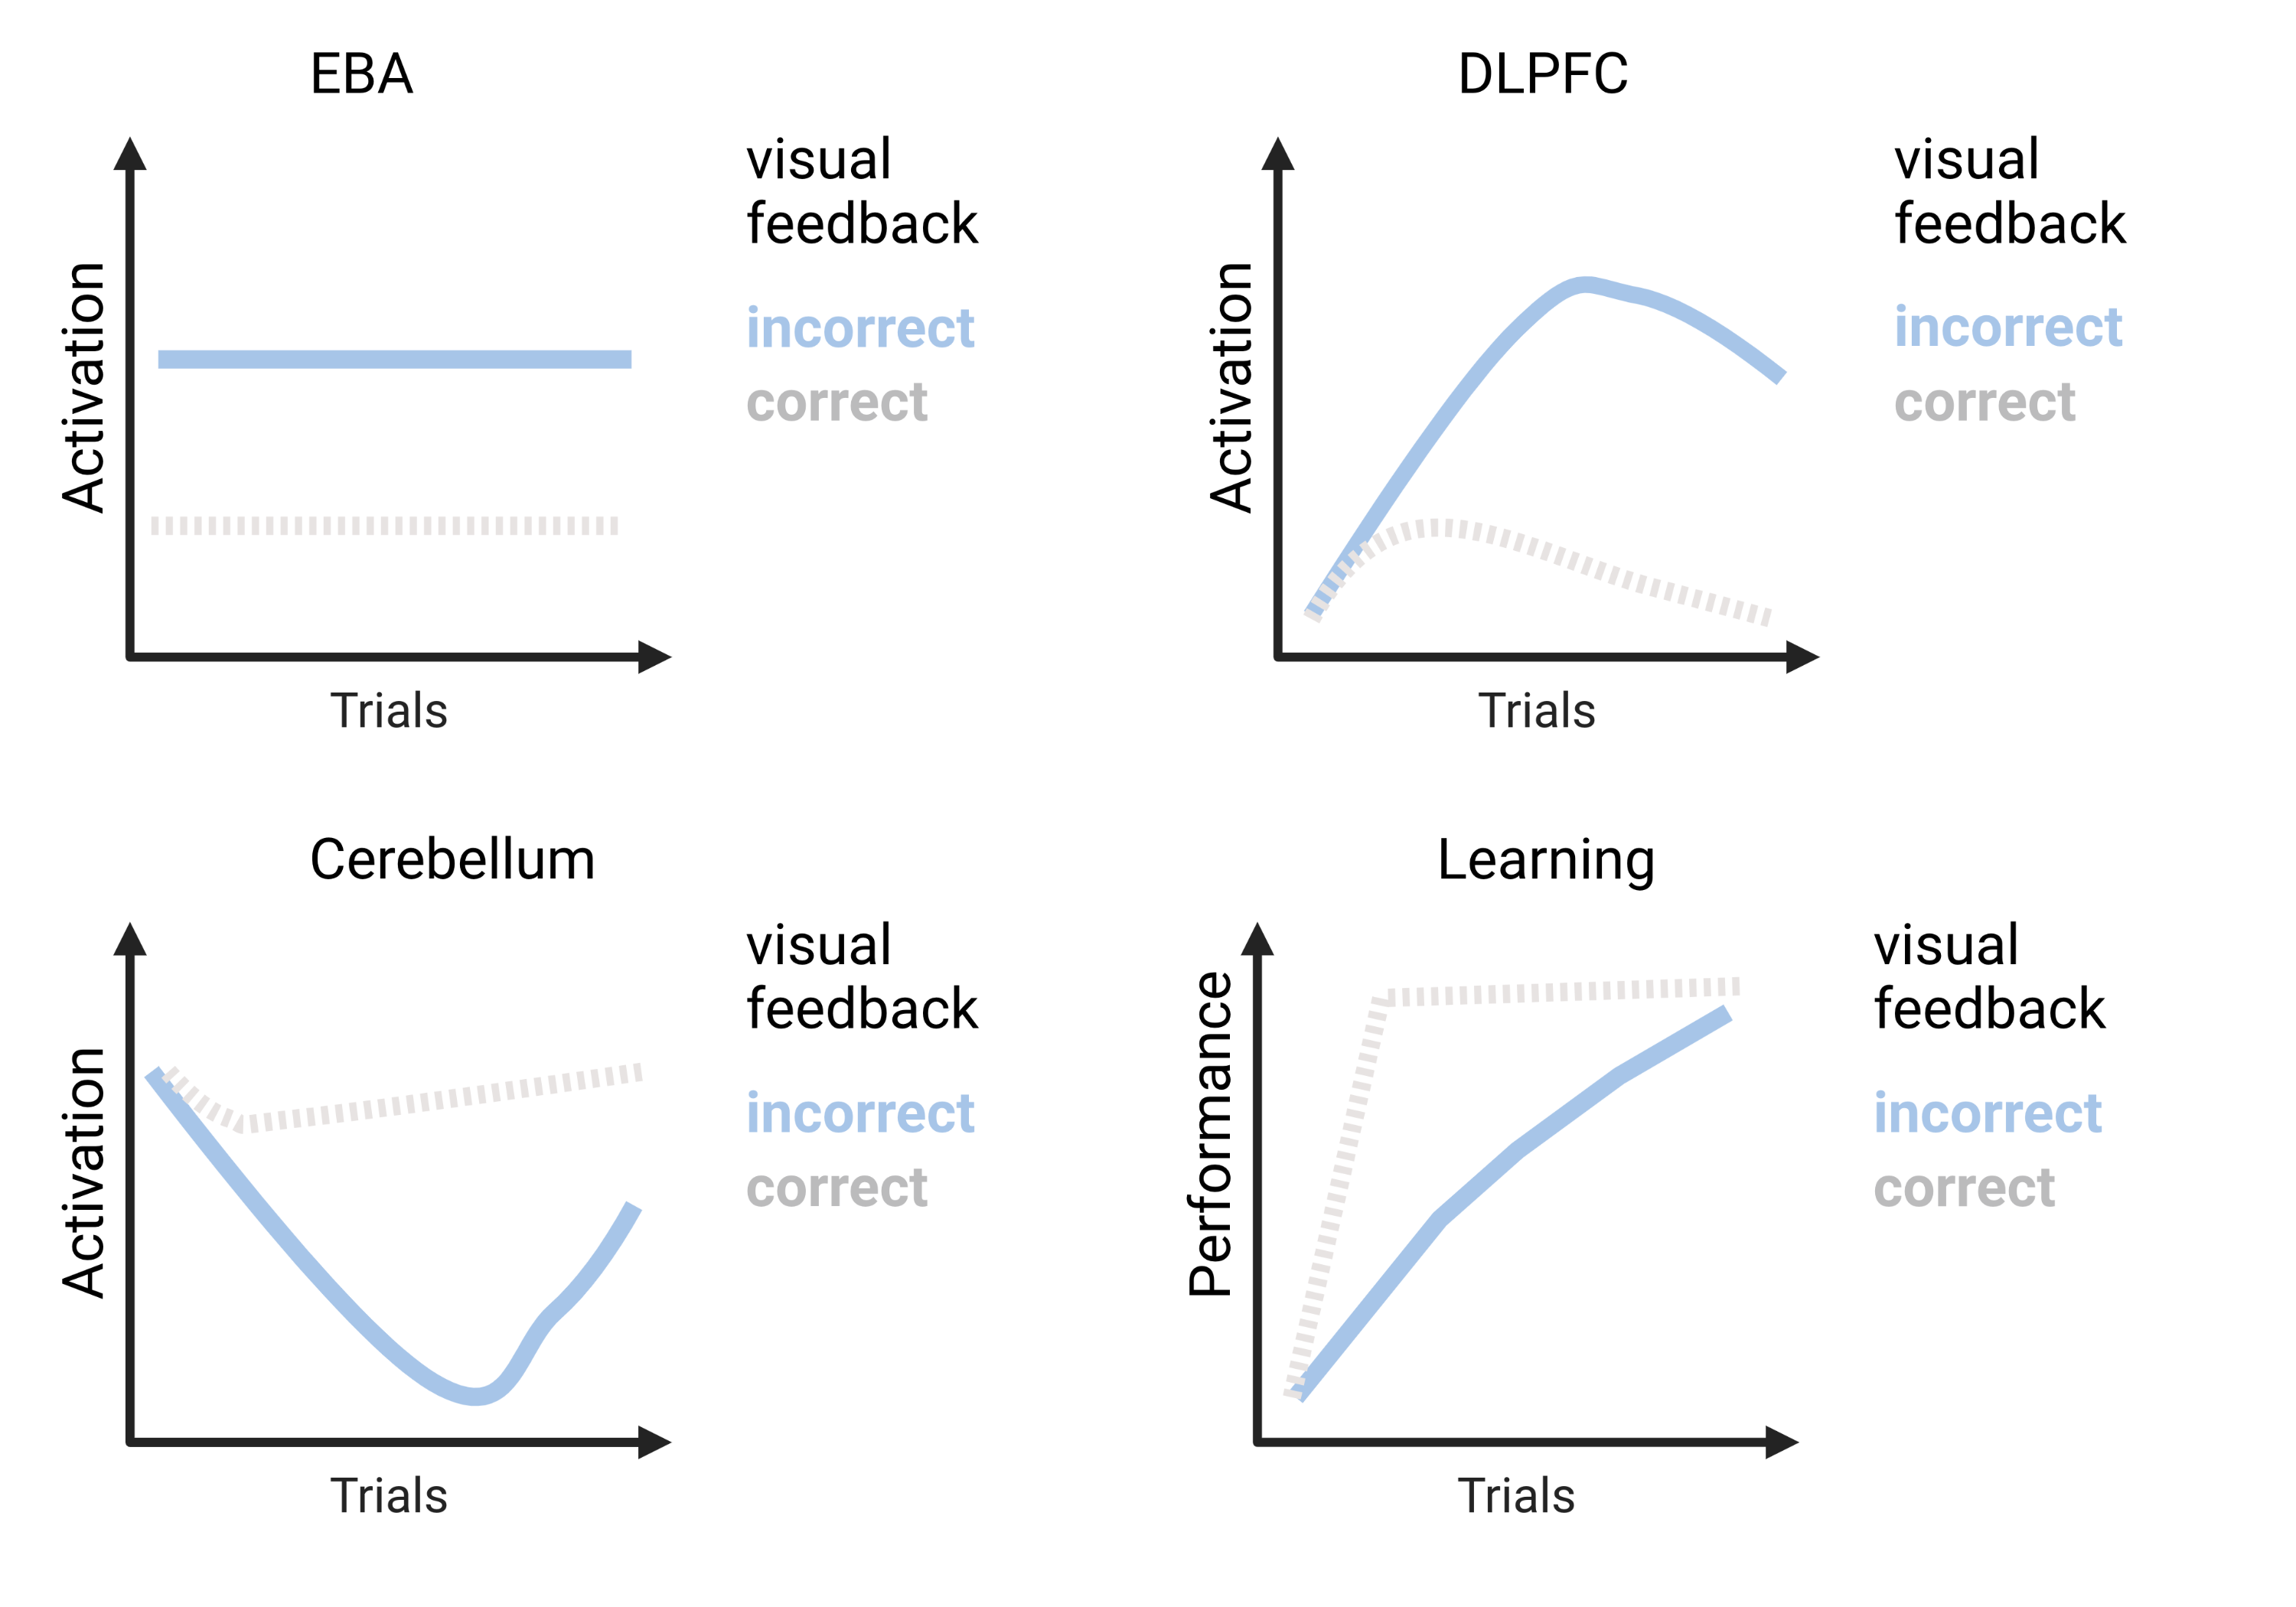
\includegraphics[width=\linewidth]{Seminar Poster/Figures/hinderance.png}
    \mbox{}\\
    \textbf{Overwrite} \\
    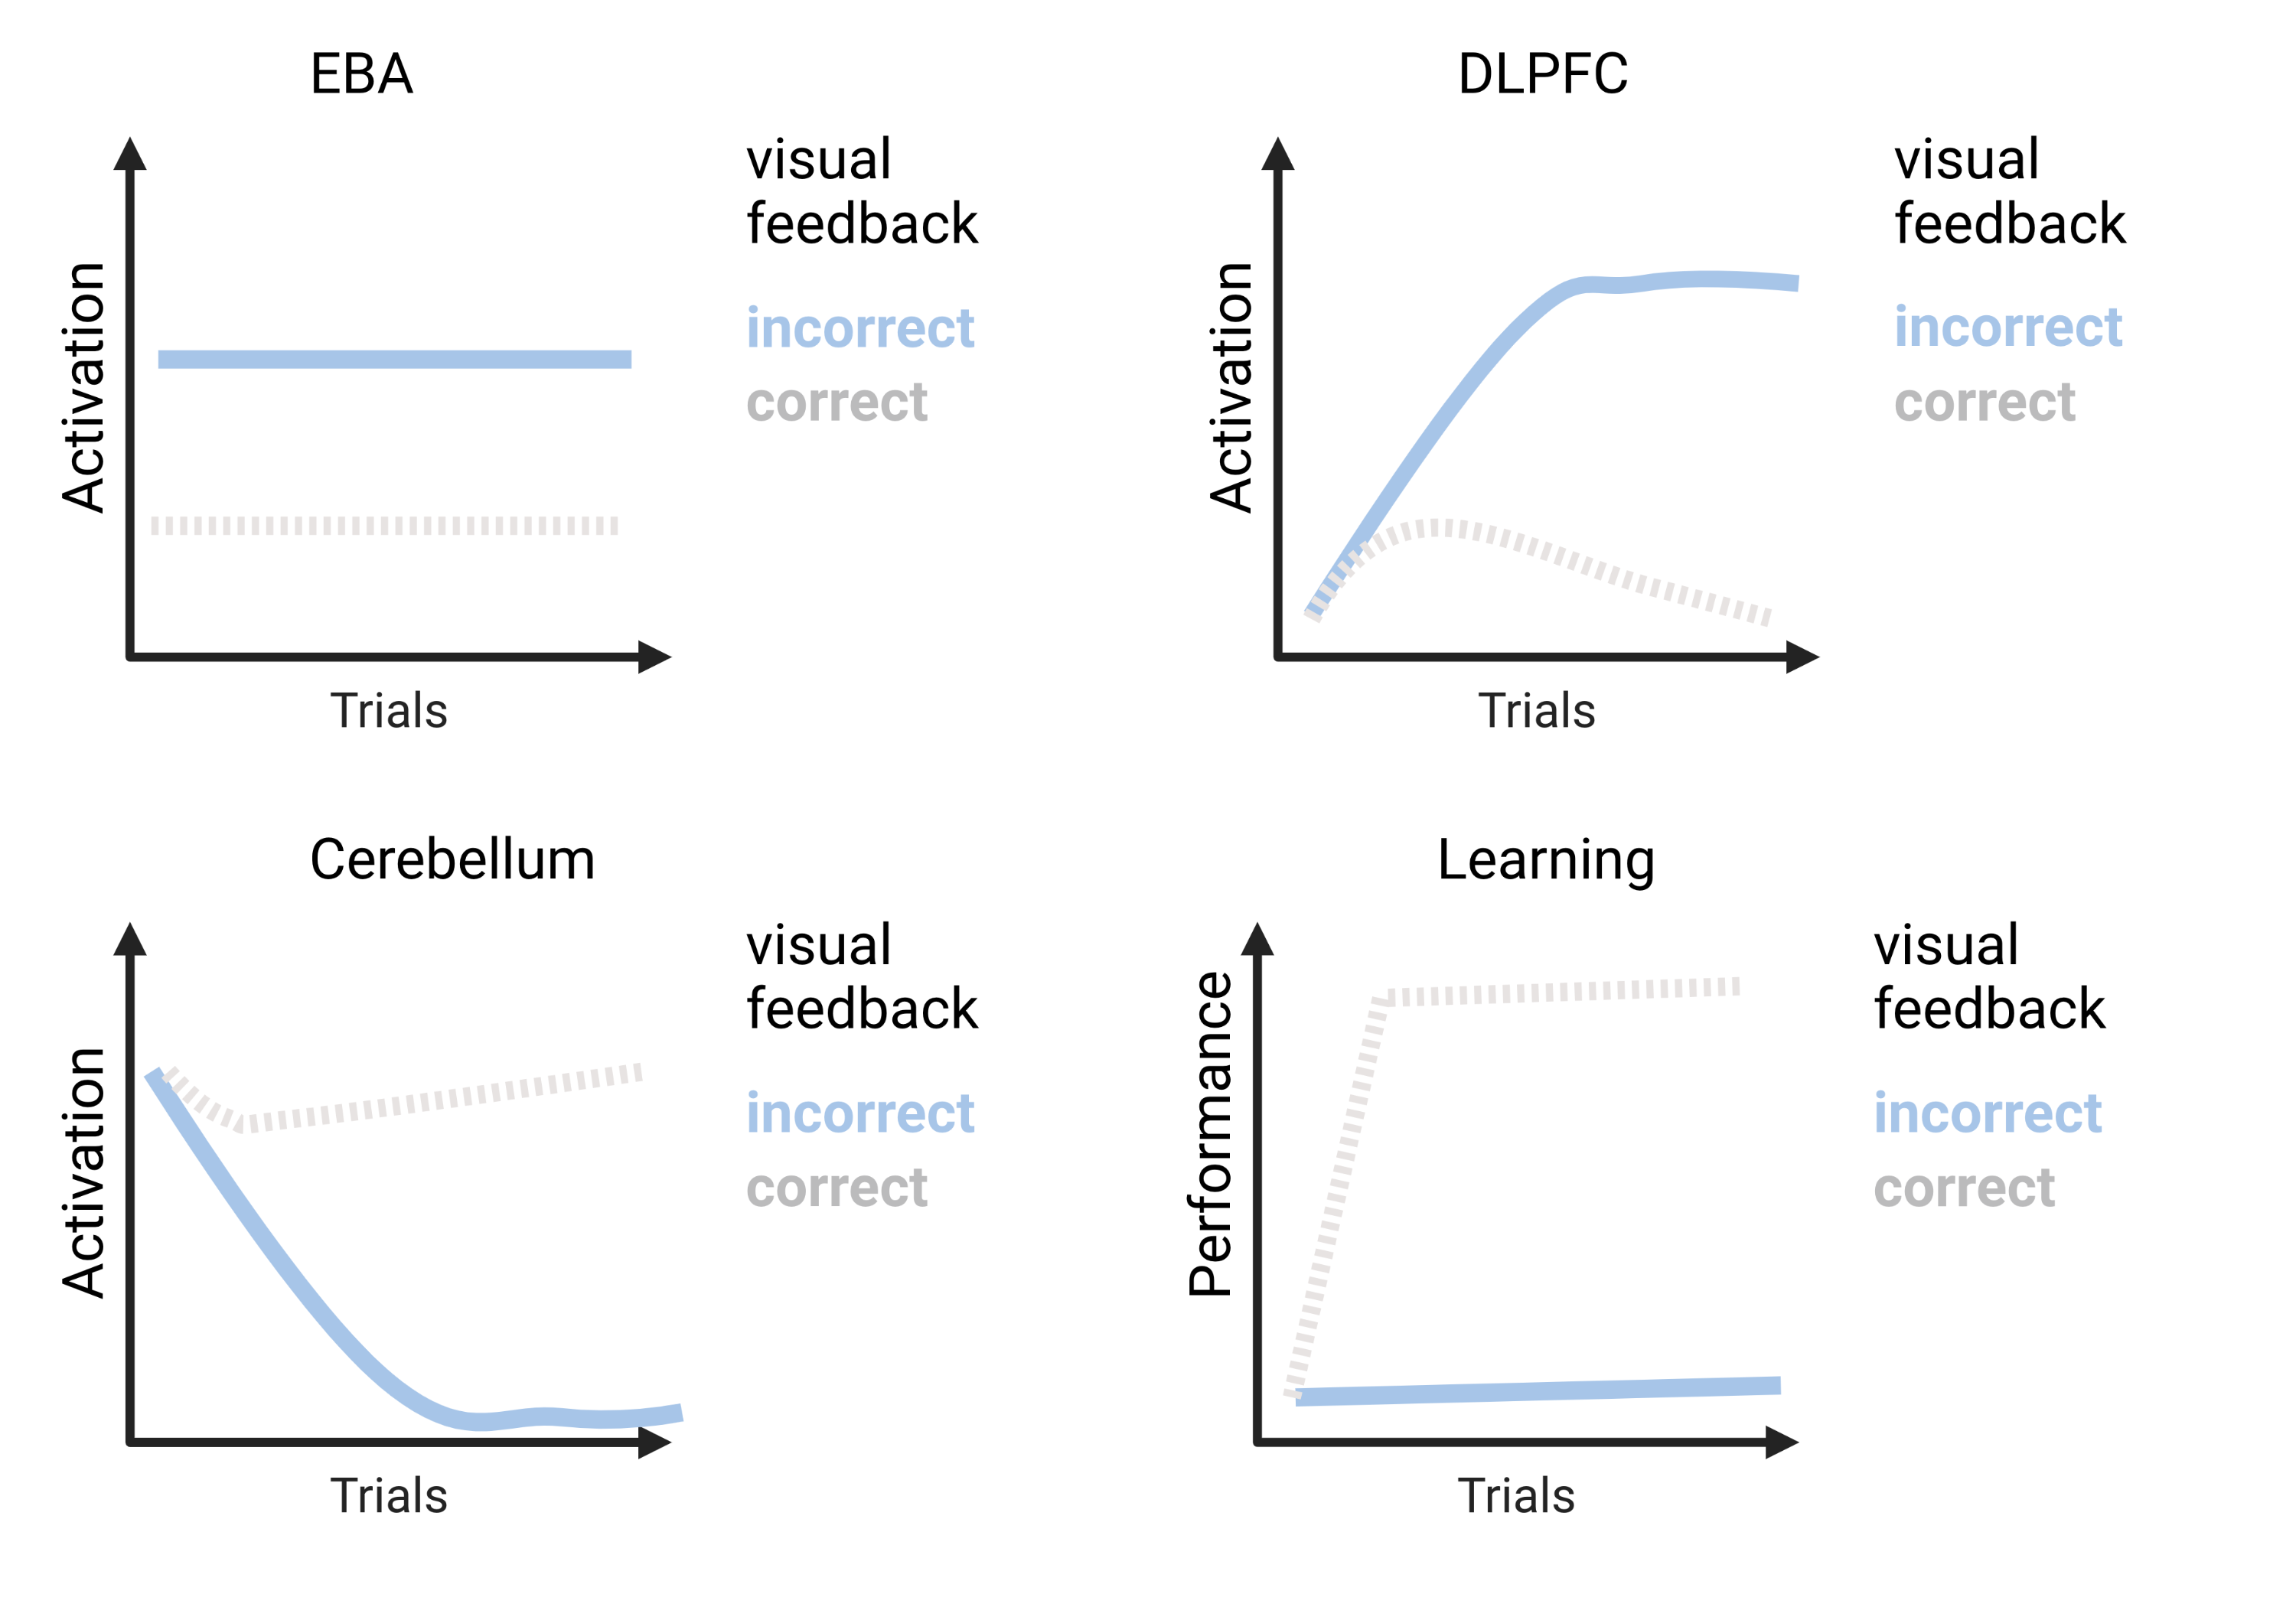
\includegraphics[width=\linewidth]{Seminar Poster/Figures/overwrite.png}
    \mbox{}\\    
    \textbf{Resilient} \\
    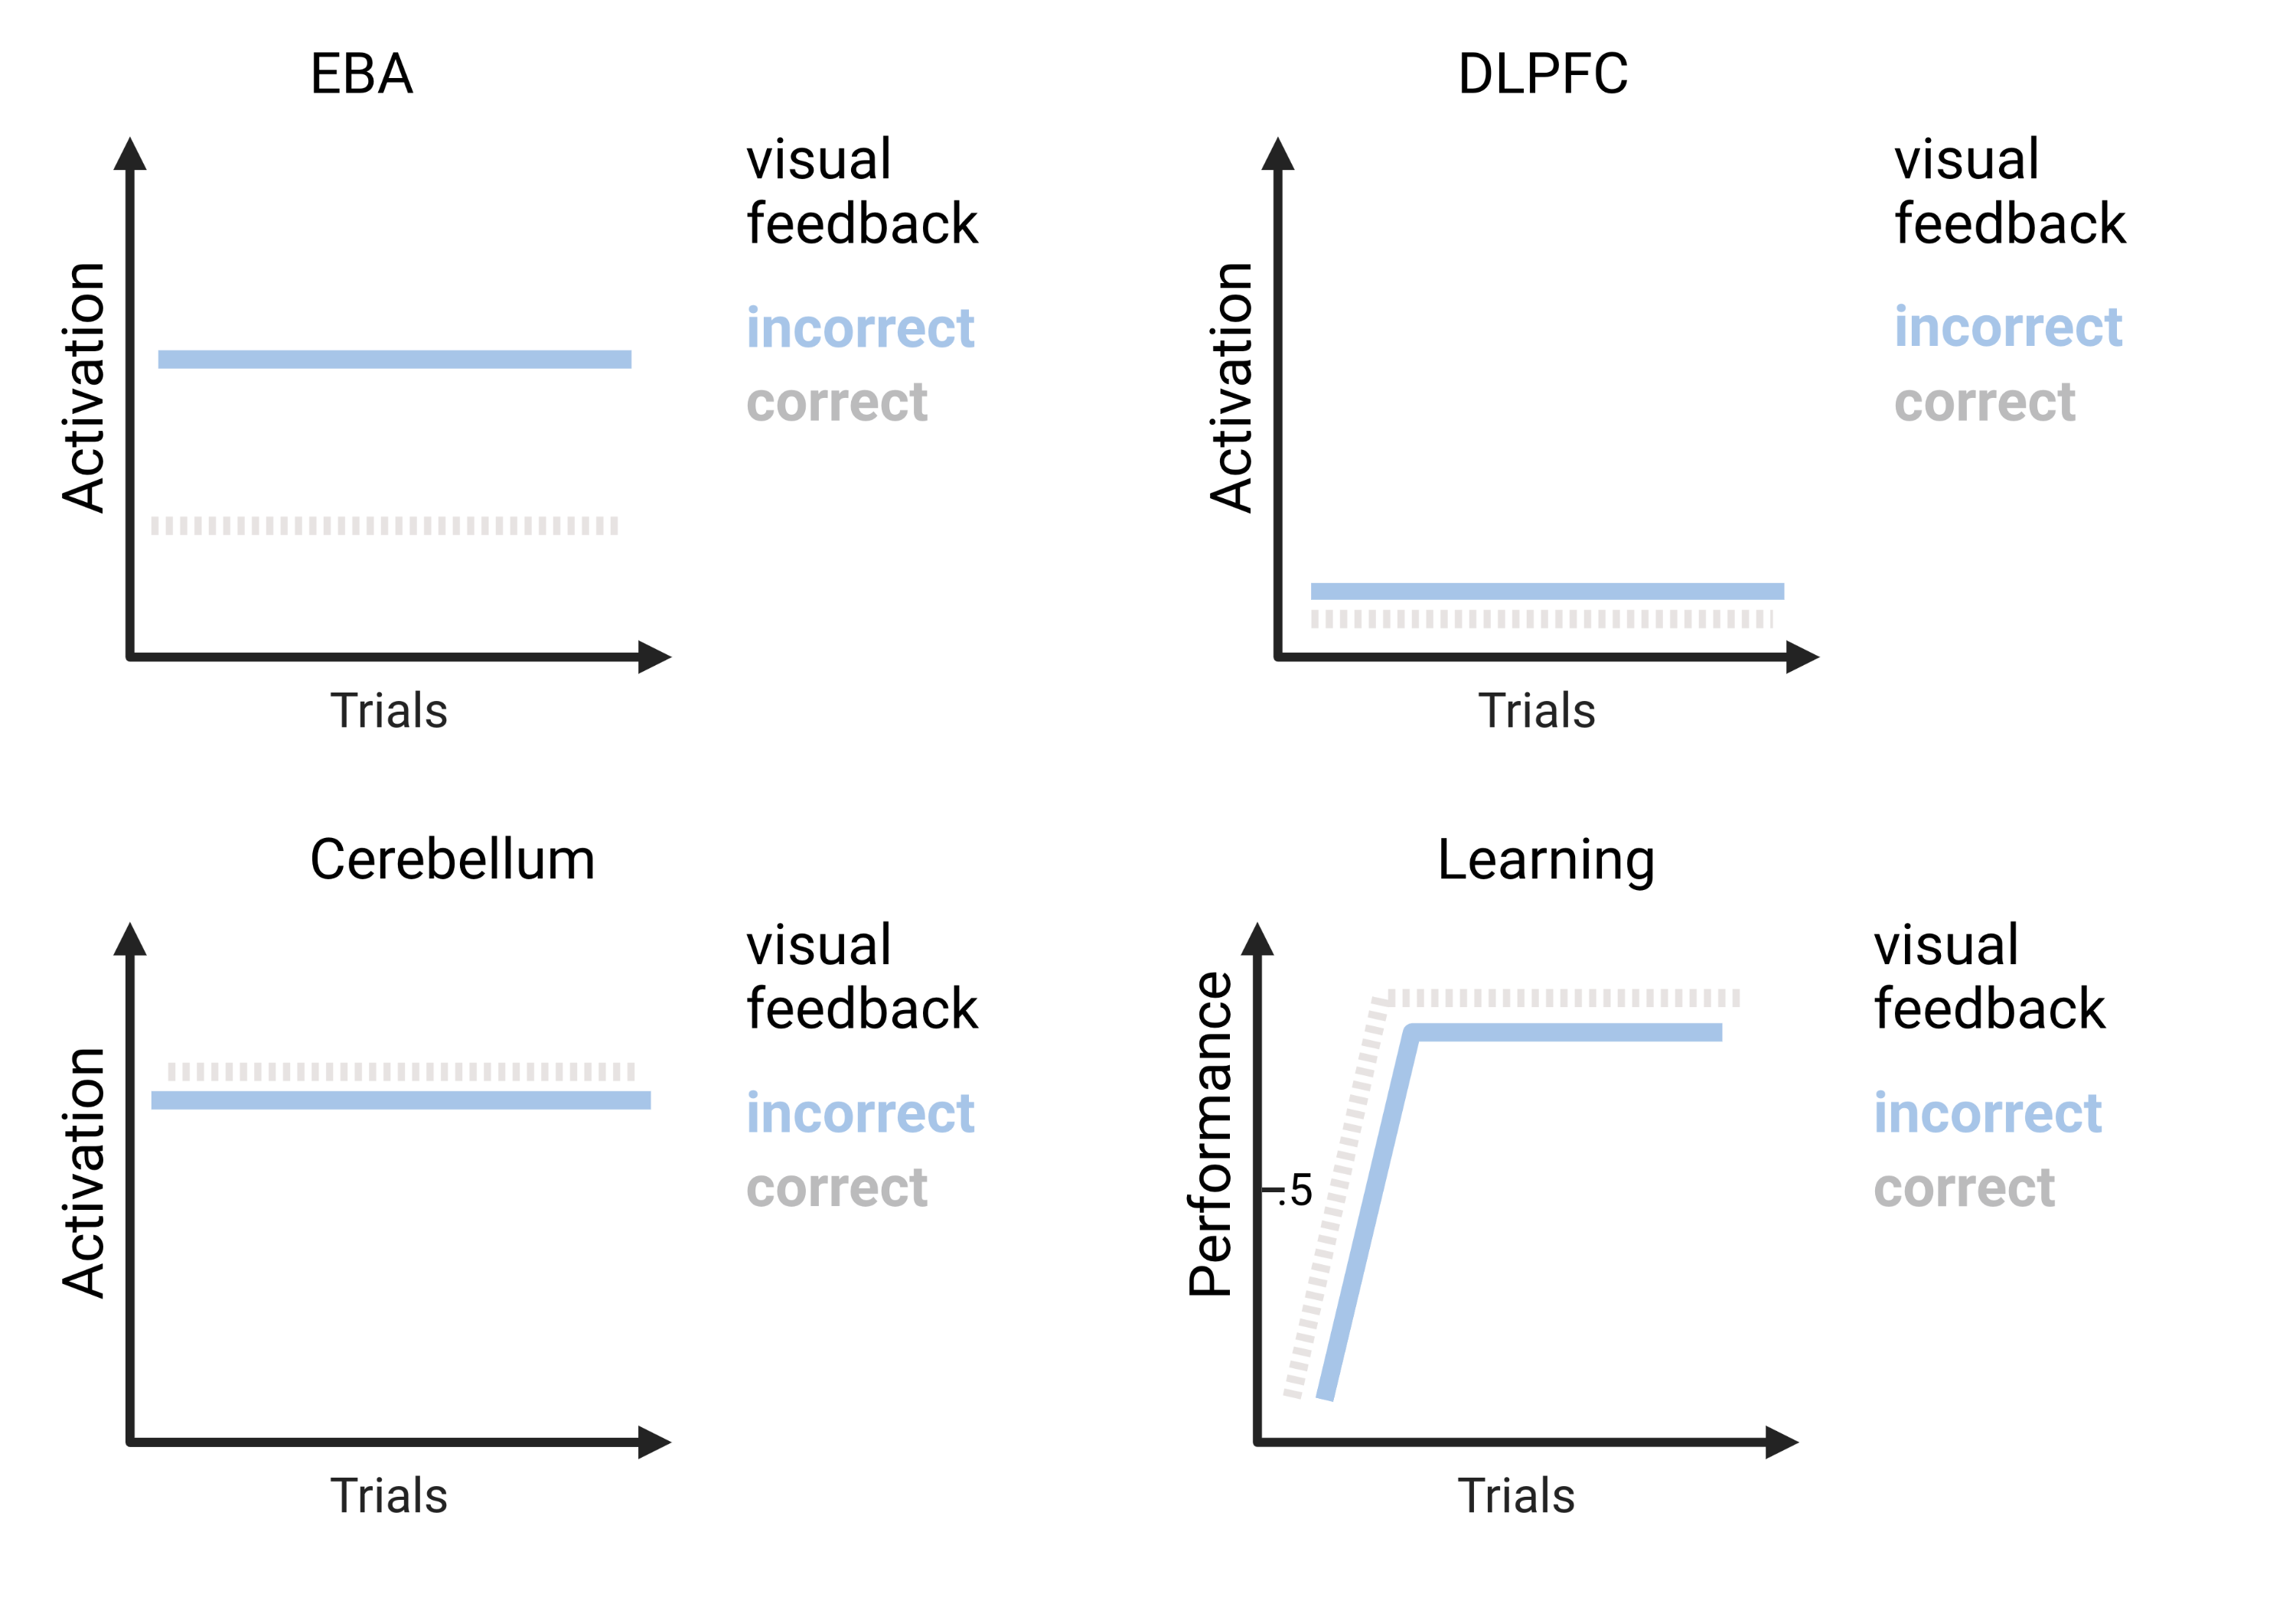
\includegraphics[width=\linewidth]{Seminar Poster/Figures/resilient.png}
    \mbox{}\\
}
%....................................................................................
%
%	Block
%
\block[titleleft,roundedcorners=16]{9. Hypothesis Confirmation}{
    \begin{itemize}
        \item \textbf{H1}: Congruency effects task performance (learning).
        \begin{itemize}
            \item Performance (negative error) significantly different for trials after correct vs incorrect feedback.
            \item \textbf{Resilient} learning model can not explain subject's performance significantly.
        \end{itemize}
        \item \textbf{H2}: Visual input can outweigh proprioceptive information.
        \begin{itemize}
            \item \textbf{Overwrite} and/or \textbf{Hinderance} learning model can explain subject's performance best.
        \end{itemize}
    \end{itemize}
 }
\end{columns} 
%..............................................................................................................................................................................................
%
%	FOOT
%
%....................................................................................
%
%	References
%
\block[titleleft,roundedcorners=16]{}{
\small
\begin{minipage}{0.73\linewidth}
	\nocite{*}
	\bibliographystyle{unsrtnat}
	\bibliography{BibPoster}
 \end{minipage}
%....................................................................................
%
%	Logos
%
\begin{minipage}{0.2\linewidth}
\centering
	
\includegraphics[height=5cm]{Figures/Logo_GitHub}
	
\includegraphics[height=5cm]{Figures/github-link-qr-code}
\end{minipage}
}
%....................................................................................
%
%	My info
%
\note[width=14cm,targetoffsetx=3cm,targetoffsety=3cm,rotate=15]{
	\textbf{Contact information:}\\
	antonio.amaddio@fu-berlin.de
}
\end{document}